\subsection{Task and Dataset}

We evaluate on the HaluEval QA split \cite{Li2023HaluEval}, which provides question--answer pairs with binary labels indicating whether the answer is correct or hallucinated. We sample 1,000 questions with balanced labels (500 correct, 500 hallucinated) to ensure that chance-level AUROC corresponds to $0.5$ and that class imbalance does not confound interpretation.

\subsection{Model}

We use Llama-3-8B-Instruct \cite{Meta2024Llama3} as the target model. This model represents the standard RLHF-fine-tuned instruction-following paradigm: it is trained with supervised fine-tuning on instruction-following data followed by RLHF alignment. We access the model through its standard Hugging Face checkpoint and apply no further fine-tuning.

\subsection{Stochastic Sampling}

For each question $q_i$, we generate a set of $N = 10$ stochastic samples:
\[
  S_i = \{s_i^{(1)}, s_i^{(2)}, \ldots, s_i^{(10)}\}
\]
using temperature $T = 1.0$, top-$p = 0.9$, and a maximum of 256 new tokens. The question is formatted using the model's standard instruction template. No ground-truth answer is provided to the model during sampling.

\subsection{SMC-NLI Score}

The NLI-based consistency score aggregates pairwise entailment and neutrality probabilities across all $\binom{10}{2} = 45$ sample pairs:

\begin{equation}
  \text{SMC-NLI}(q_i) = \frac{1}{45} \sum_{j < k} \left[ P_\text{ent}(s_i^{(j)}, s_i^{(k)}) + P_\text{neut}(s_i^{(j)}, s_i^{(k)}) \right]
\end{equation}

where $P_\text{ent}$ and $P_\text{neut}$ are the entailment and neutrality probabilities assigned by the DeBERTa NLI model \cite{He2021DeBERTa} to the ordered pair $(s_i^{(j)}, s_i^{(k)})$. A higher score indicates greater semantic consistency across samples. The score lies in $[0, 1]$ and approaches $1$ when all sample pairs are mutually entailing.

Note that we compute the score symmetrically by summing both directions of entailment and averaging; this follows the formulation in \cite{Kuhn2023Semantic} and avoids directional asymmetries in NLI scoring.

\subsection{SMC-Embed Score}

The embedding-based consistency score aggregates pairwise cosine similarities across all 45 sample pairs:

\begin{equation}
  \text{SMC-Embed}(q_i) = \frac{1}{45} \sum_{j < k} \cos\left(\mathbf{e}_i^{(j)}, \mathbf{e}_i^{(k)}\right)
\end{equation}

where $\mathbf{e}_i^{(j)}$ is the Sentence-BERT \cite{Reimers2019Sentence} embedding of sample $s_i^{(j)}$. Cosine similarity lies in $[-1, 1]$; for typical sentence embeddings it is bounded below by approximately $0$.

\subsection{Classification Protocol}

Both scores are used as hallucination detectors by thresholding: a question is predicted to be hallucinated if its consistency score falls below a threshold $\tau$. We evaluate over all thresholds using the area under the ROC curve (AUROC), which is threshold-free and summarizes discrimination ability across the full operating range. A detector with no discrimination ability achieves AUROC $= 0.5$.

\subsection{Implementation Verification}

To ensure that observed results reflect model behavior rather than implementation error, we verify our pipeline through 14 unit tests covering: (1) sampling pipeline correctness (determinism under fixed seed, output format), (2) NLI scorer correctness (expected score ordering for identical, paraphrased, and contradictory sentence pairs), (3) embedding scorer correctness (cosine similarity bounds and ordering), (4) pairwise aggregation (correct pair count, formula implementation), and (5) end-to-end score range and label alignment.

\subsection{Mechanism Verification}

Beyond unit tests, we perform a mechanism verification step that directly tests whether the NLI classifier can distinguish consistent from inconsistent pairs \emph{in principle}. We construct synthetic sentence pairs with known semantic relationships (entailment, neutral, contradiction) and confirm that the NLI model assigns scores in the expected order. This confirms that a failure in AUROC cannot be attributed to a malfunctioning NLI classifier.

\begin{figure}[t]
  \centering
  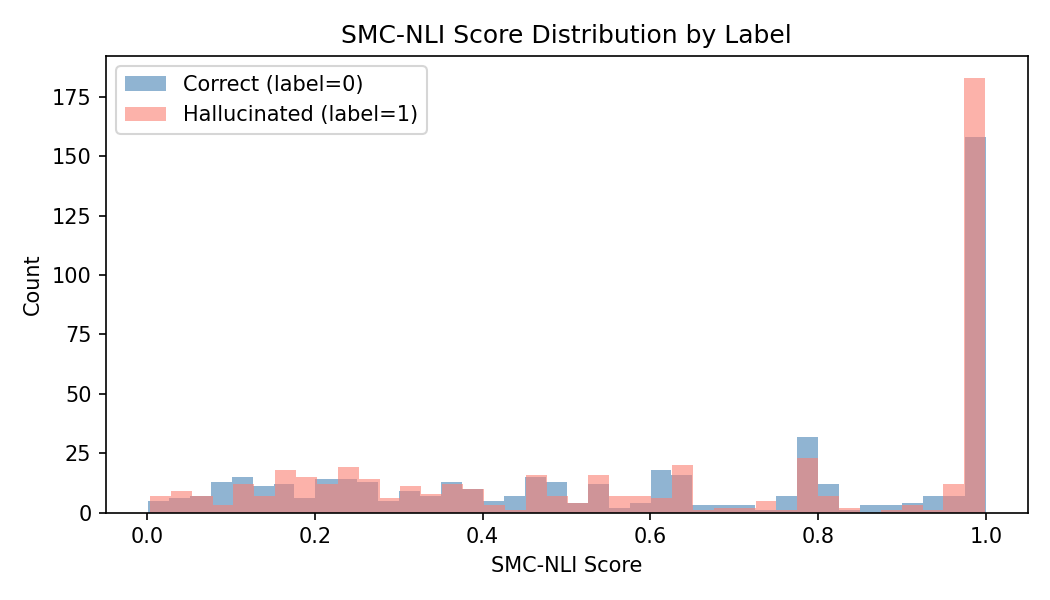
\includegraphics[width=0.45\textwidth]{figures/smc_nli_distribution}
  \caption{Distribution of SMC-NLI scores split by label (correct vs.\ hallucinated).}
  \label{fig:smc_dist}
\end{figure}

Figure~\ref{fig:smc_dist} shows the empirical distribution of SMC-NLI scores for correctly-labeled and hallucinated-labeled questions. The two distributions overlap almost completely, consistent with the near-zero mean difference reported in Section~5.

\subsection{Hyperparameters and Reproducibility}

\begin{table}[t]
  \centering
  \caption{Key hyperparameters for the SMC evaluation pipeline.}
  \label{tab:hyperparams}
  \begin{tabular}{ll}
    \toprule
    Parameter & Value \\
    \midrule
    Number of samples $N$ & 10 \\
    Sampling temperature & 1.0 \\
    Top-$p$ & 0.9 \\
    Max new tokens & 256 \\
    NLI model & \texttt{cross-encoder/nli-deberta-v3-base} \\
    Embedding model & \texttt{sentence-transformers/all-MiniLM-L6-v2} \\
    Evaluation set size & 1,000 (balanced) \\
    Random seed & 42 \\
    \bottomrule
  \end{tabular}
\end{table}

All hyperparameters are listed in Table~\ref{tab:hyperparams}. We fix the random seed to 42 for all stochastic operations. Experiments are run on a single NVIDIA A100 GPU.
